\documentclass{article}
\usepackage{tikz}
\usepackage{amssymb}
\usepackage{amsthm}
\usepackage{amsmath}
\usepackage{mathabx}
\usepackage{listings}
\usepackage{bbm}
\usepackage{caption}
\usepackage{natbib}
\usepackage{float}
\usepackage{hyperref}
\usepackage{setspace}
\usepackage[margin = 1 in]{geometry}
\usepackage{tcolorbox}
\usetikzlibrary{patterns,automata,positioning,arrows}
\title{Game Theoretical Defenses against Poisoning Attack}
\author{-}
\date{October 3, 2019}
\hbadness=99999

\begin{document}
\newtheorem{thm}{Theorem}
\newtheorem{cor}{Corollary}
\newtheorem{lem}{Lemma}
\newtheorem{prop}{Proposition}
\newtheorem{conj}{Conjecture}
\newtheorem{algo}{Algorithm}
\newtheorem{obs}{Observation}
\newtheorem{clm}{Claim}
\theoremstyle{definition}
\newtheorem{df}{Definition}
\newtheorem{eg}{Example}
\newtheorem{asm}{Assumption}
\newtheorem{cond}{Condition}
\theoremstyle{remark}
\newtheorem{rmk}{Remark}
\maketitle \onehalfspacing \allowdisplaybreaks \raggedbottom


\section{Motivation} 

\subsection{What harm does it cause?}
\begin{enumerate}
\item The loss of revenue due to the decrease in user satisfaction. Fake ratings and reviews cause customers to purchase unwanted or lower quality items, which results in low satisfaction. Unsatisfied users will often switch to alternative platforms, and this creates a significant loss of future revenue from such users.
\item The loss of advertisement revenue. The sellers may choose alternative methods of advertising, for example, through fake purchases and hiring people to generate fake reviews, over the promotion service provided by the e-commerce platform. In this case, the platform will lose a significant amount of advertisement revenue.
\end{enumerate}





\section{Game-Theoretic Approach} 

\subsection{Formal Model of the Game}
We use a Stackelberg game with incomplete information to model the situation. In this game, given a clean dataset of $n $ items, $D_{n}$, the attacker first chooses an adversarial dataset of size $k $ or less, $\Delta_{k}$, to add the items to $D_{n}$. The defender observes the combined (poisoned) dataset, $D_{n} \cup \Delta_{k}$, and sanitize it by selecting a subset $S\left(D_{n} \cup \Delta_{k}\right) $. Formally, the game can be specified by its extensive form $\Gamma = \left(N, H, P, I, u \right)$, in which,
\begin{itemize}
\item $N  = \left\{A , D \right\}$ is the set of players $A $ is the attacker, $D $ is the defender.
\item $H  = \left\{\emptyset, D_{n} \in X^{n}, \left(D_{n}, \Delta_{k}\right) \in X^{n} \times X^{\leq  k}\right\} \cup \left\{\left(D_{n}, \Delta_{k}, S\right) \in X^{n} \times X^{\leq  k} \times \left\{0, 1\right\}^{|D_{n} \cup \Delta_{k}|}\right\}$ is the set of histories including the initial history $\emptyset$, the non-terminal histories after nature's choice of $D_{n}$, and after the attacker's move $\Delta_{k}$ representing $k $ or less elements from the set of possible data items in $X $, and the terminal histories after the defender's move $S $ representing a selection of a subset of the poisoned dataset $D_{n} \cup \Delta_{k.}$
\item $I  = \left\{\emptyset\right\} \cup X^{n} \cup \left\{X^{\leq  n + k} \setminus  \sim _{I}\right\},$ where $\sim _{I}$ is the equivalence relation on the length-two histories $\left(D_{n}^{\left(1\right)} \cup \Delta_{k}^{\left(1\right)} \sim _{I} D_{n}^{\left(2\right)} \cup \Delta_{k}^{\left(2\right)}\right.$ if they are indistinguishable by the defender, for example, if these sets are just permutations of each other.
\item $P  : P\left(\emptyset\right) =$ Nature, $P\left(D_{n}\right)  = A  \;\forall\; D_{n} \in X^{n}, P\left(D_{n}, \Delta_{k}\right)  = D  \;\forall\; \left(D_{n}, \Delta_{k}\right) \in X^{n} \times X^{\leq  k}$, is the player function: nature chooses an attacker type $D_{n}$ first according to some distribution $\mathcal{F}\left(D_{n}\right)$, the attacker moves next and defender moves last after observing the information sets generated by nature and the attacker's action.
\item $u  : u_{A}\left(D_{n}, \Delta_{k}, S\right) = f\left(g\left(S\left(D_{n} \cup \Delta_{k}\right)\right) - c\left(\Delta_{k}\right), u_{D}\left(D_{n}, \Delta_{k}, S\right) = -d\left(g\left(D_{n}\right), g\left(S\left(D_{n} \cup \Delta_{k}\right)\right)\right)\right.$ is the payoff after terminal histories. In particular, the attacker gets a profit based on the parameter $\hat{\theta} = g\left(S\left(D_{n} \cup \Delta_{k}\right)\right.$ learned from the poisoned data set. Here, $g $ is the learning algorithm. The defender gets a profit based on some distance between $\hat{\theta}$ and the true parameter value $\theta^\star  = g\left(D_{n}\right)$ learned from the clean data set.
\end{itemize}


\subsection{Example}
We use the following concrete example to describe the actions and payoffs of the game. Suppose the attacker is a seller on an e-commerce platform, and the defender is the platform. Then $D_{n}$ is the set of true customer ratings of the seller's product. The possible set of ratings are $X $, for example, $X  = \left\{1, 2, 3, 4, 5\right\}$. The seller then hires $k $ or less fake customers to purchase the product and generate fake ratings $\Delta_{k} \in X^{\leq  k}$. The platform observes $D_{n} \cup \Delta_{k}$ and removes suspected fake ratings using the filter function $S  \in \left\{0, 1\right\}^{| D_{n} \cup \Delta_{k} |}$, for example, $\left\{0, 1, 0, 1, 0\right\} \in S  = \left\{0, 1\right\}^{5}$ represents removing the first, third and fifth rating from a set of five ratings. Suppose the ratings are summarized by a single number, for example the average rating $\hat{\theta} = g\left(S\left(D_{n} \cup \Delta_{k}\right)\right), g\left(\cdot \right)  = \text{\;average\;}\left(\cdot \right)$, then payoff to the seller is the revenue generated from this average, $f\left(\hat{\theta}\right) $, minus the cost of hiring fake customers, $c\left(\Delta_{k}\right) $, and the payoff to the platform is the negative revenue or loss due to the discrepancy between the poisoned average $\hat{\theta}$ and the true average $\theta^\star  = g\left(D_{n}\right), d\left(\hat{\theta}, \theta^\star \right) $, such as the loss of customers due to lower satisfaction, or the loss of reputation due to inaccurate ratings.
\newline \newline
In the simplest numerical example, $X  = \left\{0, 1\right\}, n  = k  = 1$ and,
\begin{align*}
g\left(X\right)  &= \dfrac{1}{|X|} \displaystyle\sum_{x \in X} x, 
\\ d\left(x, y\right)  &= \left| x - y \right|.
\end{align*}
Here, the ratings are either $0$ or $1$, say "dislike" or "like". The platform displays the average sanitized rating $\hat{\theta} = g\left(S\left(D_{1} \cup \Delta_{1}\right)\right)$. The ideal average for the seller is $\theta^{\dagger} = 1$. The seller wants the rating to be close to $\theta^{\dagger}$ while the platform wants the rating to be truthful $\theta^\star  = g\left(D_{1}\right)$. The prior belief of the true product rating is,
\begin{align*}
\mathbb{P}\left\{D_{1} = \left\{0\right\}\right\} &= p, 
\\ \mathbb{P}\left\{D_{1} = \left\{1\right\}\right\} &= 1 - p. 
\end{align*}
For simplicity, suppose that the cost of adding a rating that is different from the one in $D_{1}$ is $c $ and the cost of adding a rating that is the same as the one in $D_{1}$ is $0$, meaning,
\begin{align*}
c\left(\Delta_{1} = \left\{0\right\} | D_{1} = \left\{1\right\}\right)  &= c\left(\Delta_{1} = \left\{1\right\} | D_{1} = \left\{0\right\}\right)  = c  < \dfrac{1}{2} ,
\\ c\left(\cdot \right)  &= 0, \text{\;otherwise\;}.
\end{align*}
The game $\Gamma$ can then be represented by the following diagram.
\newline \newline
\begin{center} 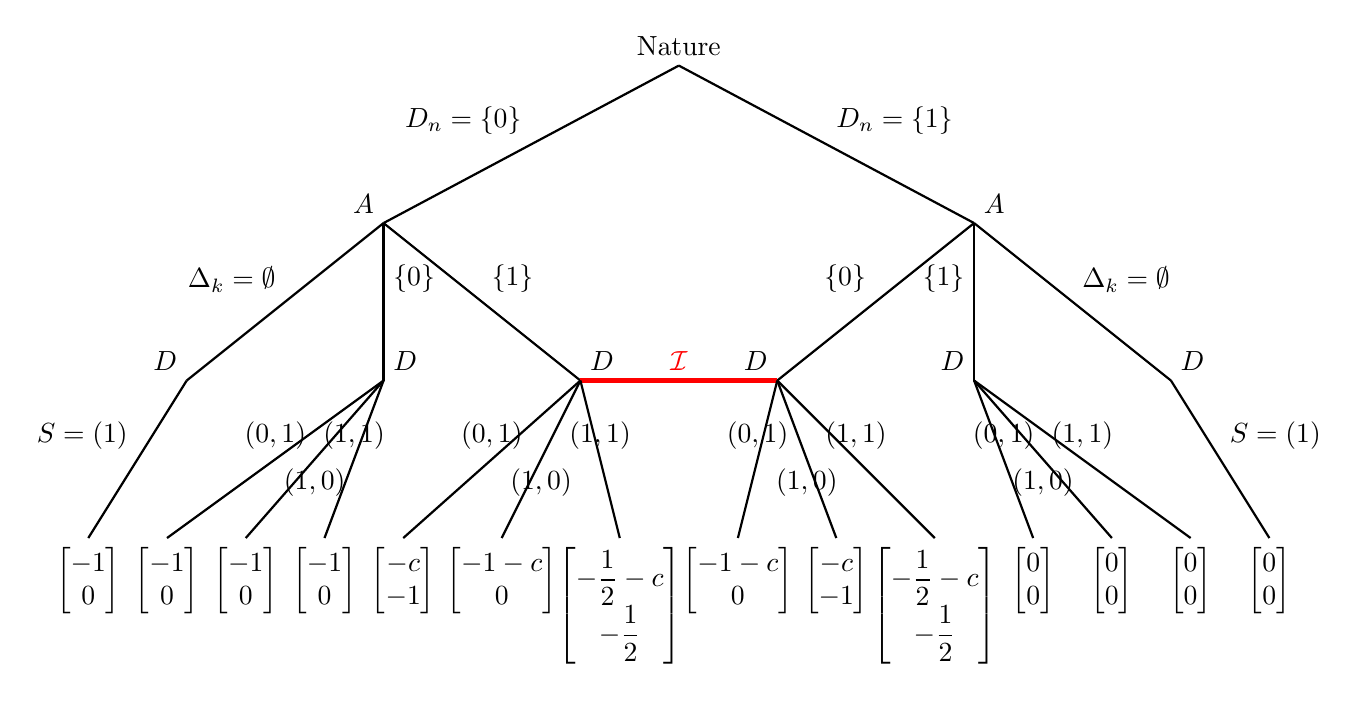
\begin{tikzpicture}[xscale = 0.25, yscale = 2.0]
\node[above] at (0.0, -1.0) {Nature};
\node[above left] at (-15.0, -2.0) {$A $};
\node[above right] at (15.0, -2.0) {$A $};
\node[above left] at (-25.0, -3.0) {$D $};
\node[above right] at (-15.0, -3.0) {$D $};
\node[above right] at (-5.0, -3.0) {$D $};
\node[above left] at (5.0, -3.0) {$D $};
\node[above left] at (15.0, -3.0) {$D $};
\node[above right] at (25.0, -3.0) {$D $};
\node[below] at (-30.0, -4.0) {$\begin{bmatrix} -1 \\ 0 \end{bmatrix}$};
\node[below] at (-26.0, -4.0) {$\begin{bmatrix} -1 \\ 0 \end{bmatrix}$};
\node[below] at (-22.0, -4.0) {$\begin{bmatrix} -1 \\ 0 \end{bmatrix}$};
\node[below] at (-18.0, -4.0) {$\begin{bmatrix} -1 \\ 0 \end{bmatrix}$};
\node[below] at (-14.0, -4.0) {$\begin{bmatrix} - c  \\ -1 \end{bmatrix}$};
\node[below] at (-9.0, -4.0) {$\begin{bmatrix} -1 - c  \\ 0 \end{bmatrix}$};
\node[below] at (-3.0, -4.0) {$\begin{bmatrix} - \dfrac{1}{2} - c  \\ - \dfrac{1}{2} \end{bmatrix}$};
\node[below] at (3.0, -4.0) {$\begin{bmatrix} -1 - c  \\ 0 \end{bmatrix}$};
\node[below] at (8.0, -4.0) {$\begin{bmatrix} - c  \\ -1 \end{bmatrix}$};
\node[below] at (13.0, -4.0) {$\begin{bmatrix} - \dfrac{1}{2} - c  \\ - \dfrac{1}{2} \end{bmatrix}$};
\node[below] at (18.0, -4.0) {$\begin{bmatrix} 0 \\ 0 \end{bmatrix}$};
\node[below] at (22.0, -4.0) {$\begin{bmatrix} 0 \\ 0 \end{bmatrix}$};
\node[below] at (26.0, -4.0) {$\begin{bmatrix} 0 \\ 0 \end{bmatrix}$};
\node[below] at (30.0, -4.0) {$\begin{bmatrix} 0 \\ 0 \end{bmatrix}$};
\draw[thick] (0.0, -1.0) -- (-15.0, -2.0);
\node[above left] at (-7.5, -1.5) {$D_{n} = \left\{0\right\}$};
\draw[thick] (0.0, -1.0) -- (15.0, -2.0);
\node[above right] at (7.5, -1.5) {$D_{n} = \left\{1\right\}$};
\draw[thick] (-15.0, -2.0) -- (-25.0, -3.0);
\node[above left] at (-20.0, -2.5) {$\Delta_{k} = \emptyset$};
\draw[thick] (-15.0, -2.0) -- (-15.0, -3.0);
\node[above right] at (-15.0, -2.5) {$\left\{0\right\}$};
\draw[thick] (-15.0, -2.0) -- (-5.0, -3.0);
\node[above right] at (-10.0, -2.5) {$\left\{1\right\}$};
\draw[thick] (15.0, -2.0) -- (5.0, -3.0);
\node[above left] at (10.0, -2.5) {$\left\{0\right\}$};
\draw[thick] (15.0, -2.0) -- (15.0, -3.0);
\node[above left] at (15.0, -2.5) {$\left\{1\right\}$};
\draw[thick] (15.0, -2.0) -- (25.0, -3.0);
\node[above right] at (20.0, -2.5) {$\Delta_{k} = \emptyset$};
\draw[red, ultra thick] (-5.0, -3.0) -- (5.0, -3.0);
\node[above, red] at (0.0, -3.0) {$\mathcal{I}$};
\draw[thick] (-25.0, -3.0) -- (-30.0, -4.0);
\node[above left] at (-27.5, -3.5) {$S  = \left(1\right)$};
\draw[thick] (-15.0, -3.0) -- (-26.0, -4.0);
\node[above] at (-20.5, -3.5) {$\left(0, 1\right)$};
\draw[thick] (-15.0, -3.0) -- (-22.0, -4.0);
\node[below] at (-18.5, -3.5) {$\left(1, 0\right)$};
\draw[thick] (-15.0, -3.0) -- (-18.0, -4.0);
\node[above] at (-16.5, -3.5) {$\left(1, 1\right)$};
\draw[thick] (-5.0, -3.0) -- (-14.0, -4.0);
\node[above] at (-9.5, -3.5) {$\left(0, 1\right)$};
\draw[thick] (-5.0, -3.0) -- (-9.0, -4.0);
\node[below] at (-7.0, -3.5) {$\left(1, 0\right)$};
\draw[thick] (-5.0, -3.0) -- (-3.0, -4.0);
\node[above] at (-4.0, -3.5) {$\left(1, 1\right)$};
\draw[thick] (5.0, -3.0) -- (3.0, -4.0);
\node[above] at (4.0, -3.5) {$\left(0, 1\right)$};
\draw[thick] (5.0, -3.0) -- (8.0, -4.0);
\node[below] at (6.5, -3.5) {$\left(1, 0\right)$};
\draw[thick] (5.0, -3.0) -- (13.0, -4.0);
\node[above] at (9.0, -3.5) {$\left(1, 1\right)$};
\draw[thick] (15.0, -3.0) -- (18.0, -4.0);
\node[above] at (16.5, -3.5) {$\left(0, 1\right)$};
\draw[thick] (15.0, -3.0) -- (22.0, -4.0);
\node[below] at (18.5, -3.5) {$\left(1, 0\right)$};
\draw[thick] (15.0, -3.0) -- (26.0, -4.0);
\node[above] at (20.5, -3.5) {$\left(1, 1\right)$};
\draw[thick] (25.0, -3.0) -- (30.0, -4.0);
\node[above right] at (27.5, -3.5) {$S  = \left(1\right)$};
\end{tikzpicture} \end{center}
The only non-singleton information set $\mathcal{I}$ is highlighted in red. The training data the defender observe when $D_{1} = \left\{0\right\}, \Delta_{1} = \left\{1\right\}$ and $D_{1} = \left\{1\right\}, \Delta_{1} = \left\{0\right\}$ are indistinguishable because they are permutations of each other. Therefore, these two histories are put in the same information set.
\newline \newline
The calculations of the payoffs for terminal histories, from left to right in the above diagram, are presented in the following table,
\begin{align*}
D' &= D_{1} \cup \Delta_{1}, S' = S\left(D'\right) .
\end{align*}
\begin{center} \begin{tabular}{|c|c|c|c|c|c|c|c|c|c|c|c|c|c|c|c|}
\hline
 $D'$ &$\left\{0\right\}$ &$\left\{0, 0\right\}$ &$\left\{0, 0\right\}$ &$\left\{0, 0\right\}$ &$\left\{0, 1\right\}$ &$\left\{0, 1\right\}$ &$\left\{0, 1\right\}$ &$\left\{0, 1\right\}$ &$\left\{0, 1\right\}$ &$\left\{0, 1\right\}$ &$\left\{1, 1\right\}$ &$\left\{1, 1\right\}$ &$\left\{1, 1\right\}$ &$\left\{1\right\}$\\ \hline
$S'$ &$\left\{0\right\}$ &$\left\{0\right\}$ &$\left\{0\right\}$ &$\left\{0, 0\right\}$ &$\left\{1\right\}$ &$\left\{0\right\}$ &$\left\{0, 1\right\}$ &$\left\{1\right\}$ &$\left\{0\right\}$ &$\left\{0, 1\right\}$ &$\left\{1\right\}$ &$\left\{1\right\}$ &$\left\{1, 1\right\}$ &$\left\{1\right\}$\\ \hline
$\hat{\theta}$ &$0$ &$0$ &$0$ &$0$ &$1$ &$0$ &$\dfrac{1}{2}$ &$1$ &$0$ &$\dfrac{1}{2}$ &$1$ &$1$ &$1$ &$1$\\ \hline
$\theta^\star $ &$0$ &$0$ &$0$ &$0$ &$0$ &$0$ &$0$ &$1$ &$1$ &$1$ &$1$ &$1$ &$1$ &$1$\\ \hline
$\theta^{\dagger}$ &$1$ &$1$ &$1$ &$1$ &$1$ &$1$ &$1$ &$1$ &$1$ &$1$ &$1$ &$1$ &$1$ &$1$\\ \hline
$\pi_{A}$ &$-1$ &$-1$ &$-1$ &$-1$ &$-c $ &$-1 - c $ &$- \dfrac{1}{2} - c $ &$-1 - c $ &$-c $ &$- \dfrac{1}{2} - c $ &$0$ &$0$ &$0$ &$0$\\ \hline
$\pi_{D}$ &$0$ &$0$ &$0$ &$0$ &$-1$ &$0$ &$- \dfrac{1}{2}$ &$0$ &$-1$ &$- \dfrac{1}{2}$ &$0$ &$0$ &$0$ &$0$\\ \hline
\end{tabular} \end{center}
\begin{center} 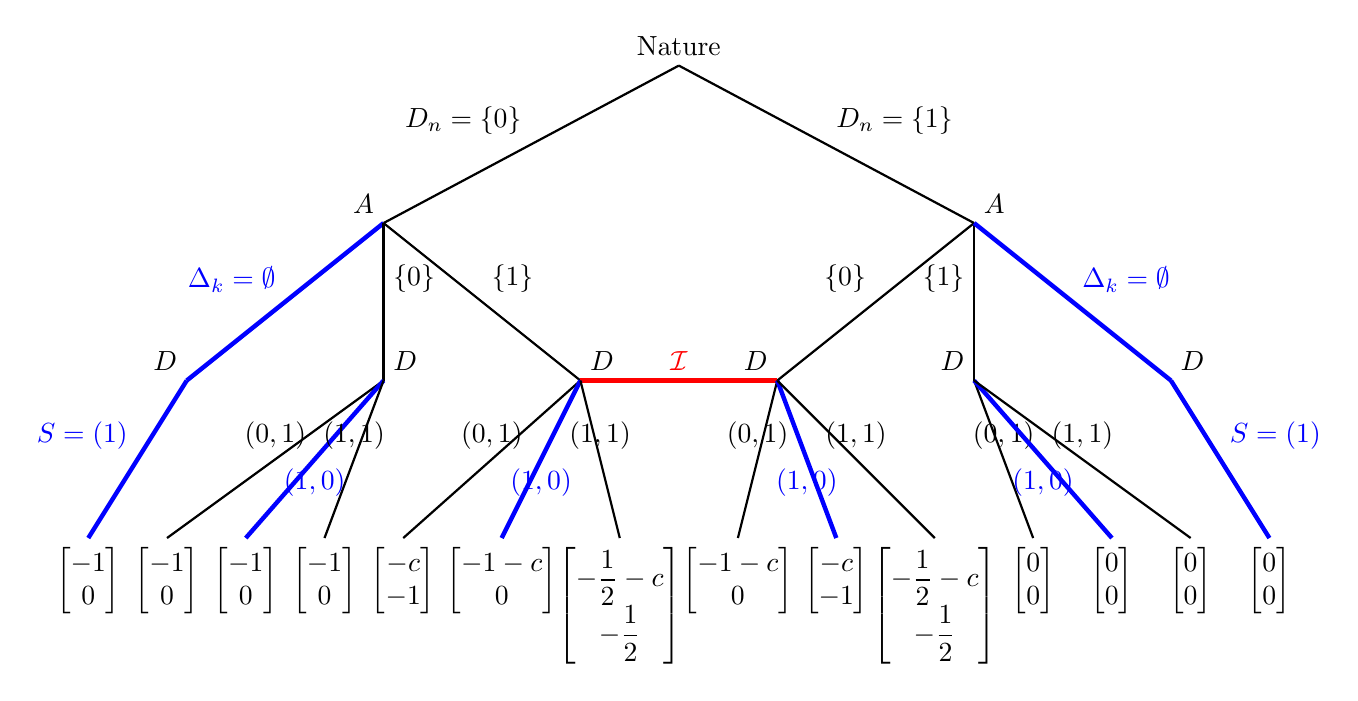
\begin{tikzpicture}[xscale = 0.25, yscale = 2.0]
\node[above] at (0.0, -1.0) {Nature};
\node[above left] at (-15.0, -2.0) {$A $};
\node[above right] at (15.0, -2.0) {$A $};
\node[above left] at (-25.0, -3.0) {$D $};
\node[above right] at (-15.0, -3.0) {$D $};
\node[above right] at (-5.0, -3.0) {$D $};
\node[above left] at (5.0, -3.0) {$D $};
\node[above left] at (15.0, -3.0) {$D $};
\node[above right] at (25.0, -3.0) {$D $};
\node[below] at (-30.0, -4.0) {$\begin{bmatrix} -1 \\ 0 \end{bmatrix}$};
\node[below] at (-26.0, -4.0) {$\begin{bmatrix} -1 \\ 0 \end{bmatrix}$};
\node[below] at (-22.0, -4.0) {$\begin{bmatrix} -1 \\ 0 \end{bmatrix}$};
\node[below] at (-18.0, -4.0) {$\begin{bmatrix} -1 \\ 0 \end{bmatrix}$};
\node[below] at (-14.0, -4.0) {$\begin{bmatrix} - c  \\ -1 \end{bmatrix}$};
\node[below] at (-9.0, -4.0) {$\begin{bmatrix} -1 - c  \\ 0 \end{bmatrix}$};
\node[below] at (-3.0, -4.0) {$\begin{bmatrix} - \dfrac{1}{2} - c  \\ - \dfrac{1}{2} \end{bmatrix}$};
\node[below] at (3.0, -4.0) {$\begin{bmatrix} -1 - c  \\ 0 \end{bmatrix}$};
\node[below] at (8.0, -4.0) {$\begin{bmatrix} - c  \\ -1 \end{bmatrix}$};
\node[below] at (13.0, -4.0) {$\begin{bmatrix} - \dfrac{1}{2} - c  \\ - \dfrac{1}{2} \end{bmatrix}$};
\node[below] at (18.0, -4.0) {$\begin{bmatrix} 0 \\ 0 \end{bmatrix}$};
\node[below] at (22.0, -4.0) {$\begin{bmatrix} 0 \\ 0 \end{bmatrix}$};
\node[below] at (26.0, -4.0) {$\begin{bmatrix} 0 \\ 0 \end{bmatrix}$};
\node[below] at (30.0, -4.0) {$\begin{bmatrix} 0 \\ 0 \end{bmatrix}$};
\draw[thick] (0.0, -1.0) -- (-15.0, -2.0);
\node[above left] at (-7.5, -1.5) {$D_{n} = \left\{0\right\}$};
\draw[thick] (0.0, -1.0) -- (15.0, -2.0);
\node[above right] at (7.5, -1.5) {$D_{n} = \left\{1\right\}$};
\draw[blue, ultra thick] (-15.0, -2.0) -- (-25.0, -3.0);
\node[above left, blue] at (-20.0, -2.5) {$\Delta_{k} = \emptyset$};
\draw[thick] (-15.0, -2.0) -- (-15.0, -3.0);
\node[above right] at (-15.0, -2.5) {$\left\{0\right\}$};
\draw[thick] (-15.0, -2.0) -- (-5.0, -3.0);
\node[above right] at (-10.0, -2.5) {$\left\{1\right\}$};
\draw[thick] (15.0, -2.0) -- (5.0, -3.0);
\node[above left] at (10.0, -2.5) {$\left\{0\right\}$};
\draw[thick] (15.0, -2.0) -- (15.0, -3.0);
\node[above left] at (15.0, -2.5) {$\left\{1\right\}$};
\draw[blue, ultra thick] (15.0, -2.0) -- (25.0, -3.0);
\node[above right, blue] at (20.0, -2.5) {$\Delta_{k} = \emptyset$};
\draw[red, ultra thick] (-5.0, -3.0) -- (5.0, -3.0);
\node[above, red] at (0.0, -3.0) {$\mathcal{I}$};
\draw[blue, ultra thick] (-25.0, -3.0) -- (-30.0, -4.0);
\node[above left, blue] at (-27.5, -3.5) {$S  = \left(1\right)$};
\draw[thick] (-15.0, -3.0) -- (-26.0, -4.0);
\node[above] at (-20.5, -3.5) {$\left(0, 1\right)$};
\draw[blue, ultra thick] (-15.0, -3.0) -- (-22.0, -4.0);
\node[below, blue] at (-18.5, -3.5) {$\left(1, 0\right)$};
\draw[thick] (-15.0, -3.0) -- (-18.0, -4.0);
\node[above] at (-16.5, -3.5) {$\left(1, 1\right)$};
\draw[thick] (-5.0, -3.0) -- (-14.0, -4.0);
\node[above] at (-9.5, -3.5) {$\left(0, 1\right)$};
\draw[blue, ultra thick] (-5.0, -3.0) -- (-9.0, -4.0);
\node[below, blue] at (-7.0, -3.5) {$\left(1, 0\right)$};
\draw[thick] (-5.0, -3.0) -- (-3.0, -4.0);
\node[above] at (-4.0, -3.5) {$\left(1, 1\right)$};
\draw[thick] (5.0, -3.0) -- (3.0, -4.0);
\node[above] at (4.0, -3.5) {$\left(0, 1\right)$};
\draw[blue, ultra thick] (5.0, -3.0) -- (8.0, -4.0);
\node[below, blue] at (6.5, -3.5) {$\left(1, 0\right)$};
\draw[thick] (5.0, -3.0) -- (13.0, -4.0);
\node[above] at (9.0, -3.5) {$\left(1, 1\right)$};
\draw[thick] (15.0, -3.0) -- (18.0, -4.0);
\node[above] at (16.5, -3.5) {$\left(0, 1\right)$};
\draw[blue, ultra thick] (15.0, -3.0) -- (22.0, -4.0);
\node[below, blue] at (18.5, -3.5) {$\left(1, 0\right)$};
\draw[thick] (15.0, -3.0) -- (26.0, -4.0);
\node[above] at (20.5, -3.5) {$\left(1, 1\right)$};
\draw[blue, ultra thick] (25.0, -3.0) -- (30.0, -4.0);
\node[above right, blue] at (27.5, -3.5) {$S  = \left(1\right)$};
\end{tikzpicture} \end{center}
One possible weak perfect Bayesian equilibrium is highlighted in blue. This equilibrium represents the case in which both types of attacker choose not to poison the dataset, meaning $\Delta_{1} = \emptyset$, and the defender always removes the higher rating if the dataset contains two ratings,
\begin{align*}
\hat{\theta} &= \displaystyle\min\left\{D_{1} \cup \Delta_{1}\right\}.
\end{align*}
Intuitively, the high type attacker (the case when nature chooses $D_{1} = \left\{1\right\}$) would never poison the dataset because poisoning would not improve her payoff, and the reason the low type attacker (the case when nature chooses $D_{1} = \left\{0\right\}$) would not poison the dataset is because the defender will remove the fake rating, so this type would prefer not to incur a wasteful cost. The defender will defend by removing the higher rating because she knows that only the low type attacker has the incentive to poison the dataset, so when she observes $D_{1} \cup \Delta_{1} = \left\{0, 1\right\}$, it must be generated by the low type attacker, so removing the $1$ is the best response. Formally, the belief when reaching the information set $\mathcal{I}$ must be,
\begin{align*}
&\mathbb{P}\left\{\left(D_{1} = \left\{0\right\}, \Delta_{1} = \left\{1\right\} | \mathcal{I}\right) = 1,\right.
\\ &\mathbb{P}\left\{\left(D_{1} = \left\{1\right\}, \Delta_{1} = \left\{0\right\} | \mathcal{I}\right) = 0.\right.
\end{align*}
It can be shown that this equilibrium (with the above belief) is also a sequential equilibrium of the game, and it satisfies the Cho-Kreps' intuitive criterion, meaning it is robust to mistakes made by either type of attacker.
\newline \newline
In general, with a more complex setting, we conjecture that there are similarly structured equilibria in which the defender can infer about the attacker's type at some information sets, and based on these posterior beliefs, deploy defense mechanisms with varying degrees. As a result, we should be able to identify a threshold $\bar{c}$ such that in equilibrium, no type of attacker would poison the dataset when the cost of generating fake ratings is higher than $\bar{c}$.
\newline \newline


\subsection{Interesting Questions}
\begin{enumerate}
\item Characterize and analyze the equilibrium strategies of the attacker and the defender for simple parameterizations of the game. For example, the action $S $ corresponding to removing extreme values from $D_{n} \cup \Delta_{k}$ could be the equilibrium action for some special class of parameterizations of the game.
\item Solve the mechanism design problem for the defender. For example, the defender can increase the (opportunity) cost of hiring fake reviewers by decreasing the advertising price on the platform. In this case, we attempt to find conditions on $c $ such that $\Delta_{k} = \emptyset$ is on the equilibrium path, meaning that the attacker will choose not to attack in equilibrium.
\end{enumerate}



\end{document}
